\section{Auswertung}
\label{sec:Auswertung}
In der folgenden Tabelle sind alle Messwerte aufgeführt \\
\begin{table}
  \centering
  \begin{tabular}{c c c c c c}
    \toprule
    Zeit/min & $T_1/K$ & $T_2/$ & $p_a/\text{bar}$ & $p_b/\text{bar}$ & $N/W$ \\
    \midrule
    0 &  21.7  & 21.9 &  5.1 &  5.2  & 170 \\
    1 &  22.1  & 21.8 &  2.4 &  7.0  & 170 \\
    2 &  23.3  & 21.8 &  2.8 &  7.2  & 180 \\
    3 &  24.6  & 20.9 &  3.0 &  7.7  & 190 \\
    4 &  26.2  & 19.4 &  3.1 &  8.2  & 195 \\
    5 &  28.0  & 17.6 &  3.1 &  8.3  & 200 \\
    6 &  29.9  & 15.8 &  3.1 &  9.0  & 200 \\
    7 &  32.0  & 14.1 &  3.1 & 10.0  & 205 \\
    8 &  35.1  & 12.3 &  3.1 & 10.5  & 205 \\
    9 &  37.5  & 10.7 &  3.1 & 10.9  & 208 \\
   10 &  36.9  &  9.0 &  3.1 & 10.4  & 210 \\
   11 &  38.8  &  7.4 &  3.1 & 11.7  & 208 \\
   12 &  40.4  &  6.0 &  3.1 & 11.0  & 208 \\
   13 &  42.1  &  4.4 &  3.1 & 11.4  & 210 \\
   14 &  43.6  &  3.0 &  3.1 & 11.9  & 210 \\
   15 &  45.2  &  1.6 &  3.2 & 12.0  & 210 \\
   16 &  46.7  &  0.5 &  3.2 & 12.5  & 210 \\
   17 &  48.0  & -0.3 &  3.2 & 13.0  & 210 \\
   18 &  49.5  & -0.7 &  3.2 & 13.1  & 210 \\
   19 &  50.7  & -1.0 &  3.2 & 13.5  & 210 \\
   \bottomrule
  \end{tabular}
  \caption{Messdatentabelle.}
  \label{tab:Data}
\end{table}

Die Temperaturverläufe sind in dem folgenden Diagramm dargestellt und mit einer
linearen Ausgleichstrechnung approximiert.
\subsection{Temperaturausgleichskurve}
\begin{figure}
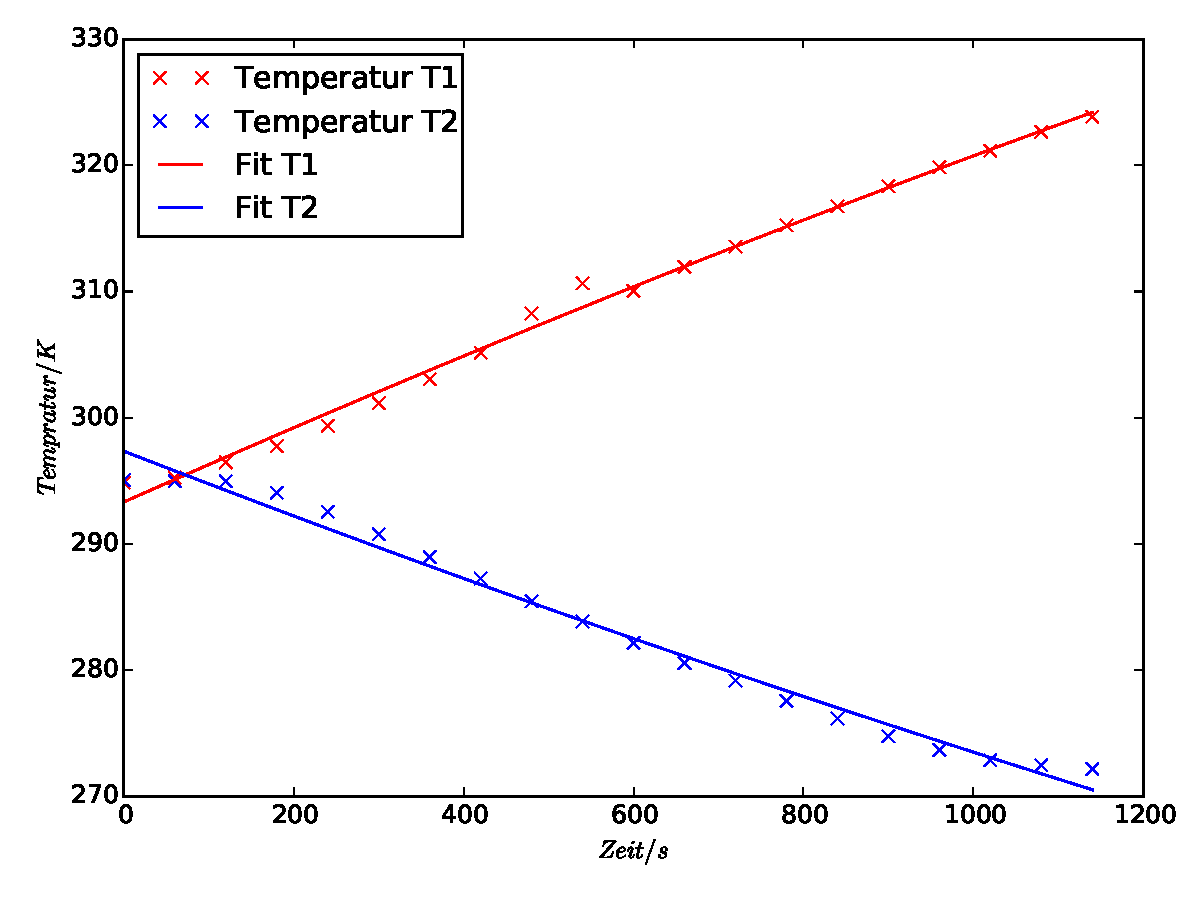
\includegraphics[height=13cm]{Temperaturgraphik.pdf}
\caption{Temperturausgleichskurve.}
\end{figure}

Die Näherung wurde mit scientific Python gemacht und ist gegeben durch
\begin{equation}
  T(t)=At^2+Bt+C .
\end{equation}
Die Parameter für erwärmte Reservoir $T_1$ sind

  $A=(-0.000002485)\frac{K}{s^2}$

  $B=(0.029925168)\frac{K}{s}$

  $C=(293.312793014)K$

Die Parameter für den anderen Behälter $T_2$ sind

  $A=(0.000002259)\frac{K}{s^2}$

  $B=(-0.026112097)\frac{K}{s}$

  $C=(297.339350549)K$

Die dazugehörigen Differentialquotienten erhält man durch die folgende Gleichung
\begin{equation}
\frac{dT}{dt}=2At+B
\end{equation}

\begin{table}
  \centering
  \begin{tabular}{c c c}
    \toprule
    $Zeit/s$ & $dT_1 /dt$ & $dT_2 /dt$ \\
    \midrule
    300  &  0.028 & -0.024  \\
    600  &  0.027 & -0.023  \\
    900  &  0.025 & -0.022  \\
   1140  &  0.024 & -0.020  \\
   \bottomrule
 \end{tabular}
 \caption{Differentialquotienten.}
 \label{tab:Diffquo}
\end{table}
\subsection{Güteziffer}
Als nächstes soll die Güteziffer bestimmt werden dafür Nutzt man die Gleichung
\eqref{eqn:gueteziffer_ideal} für die ideale Güteziffer und die Gleichung
\eqref{eqn:gueteziffer_real}
\begin{table}
  \centering

  \begin{tabular}{c c c}
    \toprule
    $Zeit/s$ & $v_\symup{ideal}$ &  $v_\symup{real}$ \\
    \midrule
      300  &  28.956  &  1.875 \\
      600  &  11.112  &  1.692 \\
      900  &  7.301  &  1.598 \\
     1140  &  6.264  &  1.523 \\
   \bottomrule
 \end{tabular}
 \caption{Güteziffer}
 \label{tab:Gütez}
\end{table}
\subsection{Massendurchsatz}
Wenn man die Werte in Gleichung \eqref{eqn:massendurchsatz} einsetzt erhält man
den Massendurchsatz.
\begin{table}
  \centering
\begin{tabular}{c c c}
  \toprule
  $Zeit /s$ & $\frac{dQ_2}{dt}$ & $\frac{dm}{dt} /\frac{mol}{s}$  \\
  \midrule
  300  &   -326.430  & -0.014  \\
  600  &   -308.554  & -0.013  \\
  900  &   -290.679  & -0.012  \\
 1140  &   -276.379  & -0.012  \\
 \bottomrule
\end{tabular}
\caption{Massendurchsatz}
\label{tab:Massend}
\end{table}
\subsection{Mechanischekompressorleistung}
Die Dichte $\rho$, die für die Berechnung mechanischen Kompressorleistung
benötigt wird, kann berechnet werden, indem man die Gleichung der idealen Gase
umstellt.
\begin{equation}
  pV=nRT \leftrightarrow \frac{pV}{T}=nR
\end{equation}
Damit ergibt sich, da die Stoffmenge $n$ konstant bleibt,
\begin{equation}
  n_1=n_2
  \frac{p_0 V_0}{T_0}=\frac{p_2 V_2}{T_2}
\end{equation}
Da $ \rho V=m$ \leftrightarrow $V= \frac{m}{\rho}$ lässt sich \rho bestimmen wobei
$\rho_2=\rho$ und $p_2=p_a$.
\begin{equation}
  \rho=\frac{\rho_0 T_0 p_a}{T_2 p_0}
\end{equation}
Und mit Gleichung \eqref{eqn:kompressorleistung}
\begin{equation}
N_\symup{mech}=\frac{1}{\kappa-1}\left(p_b \sqrt[\kappa]{\frac{p_a}{p_b}}-p_a\right)\frac{1}{\frac{\rho_0 T_0 p_a}{T_2 p_0}}\frac{dm}{dt}
\end{equation}

\begin{table}
  \centering
\begin{tabular}{c c c}
  \toprule
  $Zeit /s$ & Dichte$\rho/\frac{g}{m^3}$ & Leistung$N_\symup{mech} /W$  \\
  \midrule
  300  &   15.49  &  -0.0026 \\
  600  &   15.05  &  -0.0031 \\
  900  &   15.13  &  -0.0033 \\
 1140  &   21.65  &  -0.0024 \\
 \bottomrule
\end{tabular}
\caption{Massendurchsatz}
\label{tab:Massend}
\end{table}
